% MODULE 8: N-HOP RESULTS ON THE FULL IEEE-39. Panel box (reference px): x 405-756, y 796.5-1129.5, title bar to y 822.5.
% Design v3: hero = spillover plot drawn thick with direct value labels and the big number 11/12; authority plot smaller; repair card; one HeroBox; NextChip.
% Text edge x = 416, right edge x = 745 (box 405-756).
% Plots: figures/module8/make_m8_plotA.py (329x58 px slot) and make_m8_plotB.py (329x102 px slot) read research/nhop_ieee39_20261006/derived/ (frozen graph = primary).
\begin{scope}
  % ---------------------------------------------------------------- tag row
  \node[anchor=west,inner sep=0pt,text=PGreen,font=\FiraSemi\fontsize{19pt}{19pt}\selectfont] at (416,835) {Full IEEE-39, exact delay 44\,ms}; % source: REPORT_E1_E2_E5.md (targets at 44 ms)
  \node[anchor=east,fill=PNavy,text=white,rounded corners=2.4mm,inner xsep=5pt,inner ysep=3pt,font=\FiraBold\fontsize{15.5pt}{15.5pt}\selectfont\addfontfeature{LetterSpace=6}] at (745,835) {NUMERICAL OBSERVATION};

  % ---------------------------------------------------------------- B: spillover (hero)
  \SectionRule{B}{Spillover on other roots}{416}{856}{554}
  % legend on the heading row: no box, just the two marks
  \fill[PRed] (556,852.5) rectangle (564,860.5);
  \node[anchor=west,inner sep=0pt,text=PRed,font=\FiraSemi\fontsize{17.5pt}{17.5pt}\selectfont] at (571,856.5) {absolute gains};
  \fill[PNavy] (652,856.5) -- (657,851.5) -- (662,856.5) -- (657,861.5) -- cycle;
  \node[anchor=west,inner sep=0pt,text=PNavy,font=\FiraSemi\fontsize{17.5pt}{17.5pt}\selectfont] at (665,856.5) {baseline + change};
  % source: derived/E5_spillover.csv (graph=frozen): 12 exact assignments (eps <= 1e-8), N_margin > 0 in 11 (absolute and delta variants); baseline 10 roots beyond -0.05.
  %   All graphs and variants: 56 of 62 leave roots beyond the margin (REPORT_E1_E2_E5.md; verified by count of spill_beyond_margin = True).
  \node[anchor=north west,inner sep=0pt] at (416,864) {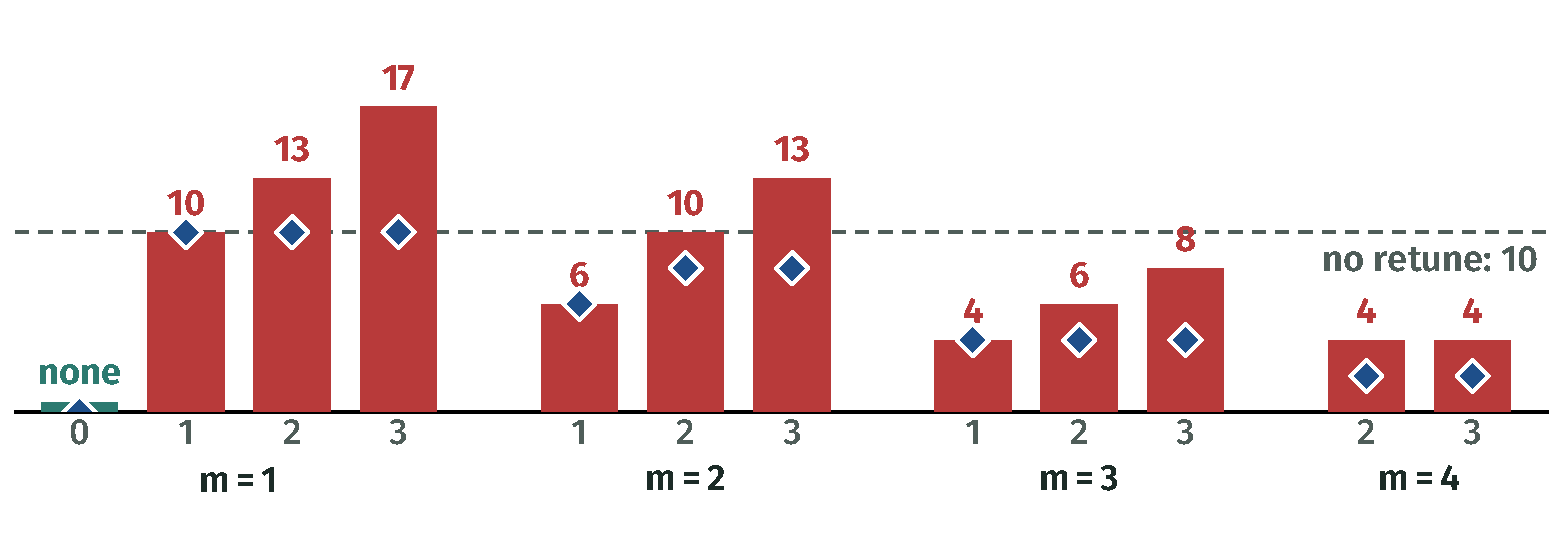
\includegraphics[width=329\PX,height=102\PY]{figures/module8/m8_plotB.pdf}};
  % statement in the empty upper right of the plot (source: E5_spillover.csv, graph=frozen: N_margin > 0 in 11 of 12 exact assignments; baseline 10 roots beyond -0.05)
  \node[anchor=north west,inner sep=0pt,text=PRed,align=left,font=\FiraSemi\fontsize{18pt}{20pt}\selectfont] at (600,872)
    {11 of 12 exact assignments leave\\roots beyond the $-0.05\,\mathrm{s^{-1}}$ margin\\(no retune: 10).};

  % ---------------------------------------------------------------- A: authority (smaller)
  \begin{scope}[shift={(0,-18)}]
  \SectionRule{A}{Authority: residual vs radius}{416}{993}{745}
  % source: derived/E1_residuals.csv (graph=frozen, eps by m, n) and E1_nmin.csv: n_min = 0, 1, 1, 2 for m = 1..4; m = 5 not reached (eps = 4.816e-4 at n = 3)
  \node[anchor=north west,inner sep=0pt] at (416,1001) {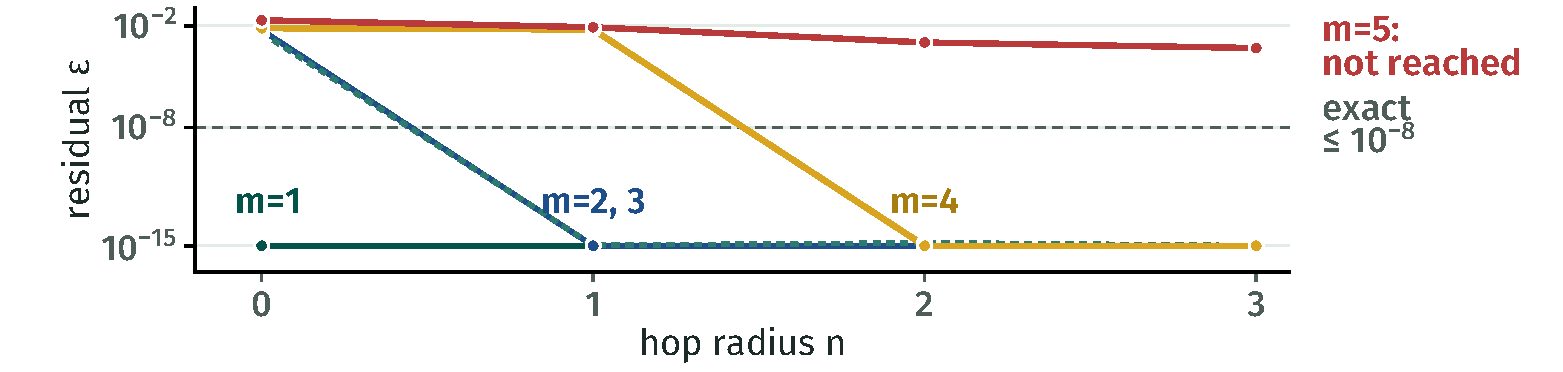
\includegraphics[width=329\PX,height=58\PY]{figures/module8/m8_plotA.pdf}};
  \node[anchor=west,inner sep=0pt,text=PMuted,font=\FiraMed\fontsize{17.5pt}{17.5pt}\selectfont] at (416,1066)
    {Each extra mode pinned needs more measured neighbors ($2m\le 2|\mathcal N_i|$).};

  % ---------------------------------------------------------------- repair card (E3/E4)
  \CardBox{416}{1074}{745}{1100}
  % source: derived/E3_repair.csv (frozen, rho 0.875: n = 0 succeeds at tau 44, 48, 52 ms; frozen n = 2 stalls at 52 ms), E4_largest_rho.csv (0.9 for every n; 0.925 and 0.95 fail for every n)
  \node[anchor=west,inner sep=0pt,text=PText,font=\FiraMed\fontsize{17.5pt}{19pt}\selectfont] at (424,1087)
    {\parbox{322\PX}{\raggedright Spectral repair at 44--52 ms already works with $n=0$; the clean-spectrum share is 90\,\% for every $n$ (events fail there, panel 9) and 92.5\,\% fails. Declared sweep, not an optimum.}};

  % ---------------------------------------------------------------- the one HeroBox
  \HeroBox{416}{1102.5}{745}{1126.5}
  \node[anchor=west,inner sep=0pt,text=PGreen,align=left,font=\FiraBold\fontsize{20pt}{21.5pt}\selectfont] at (427,1114.5) {Exact assignment of selected modes does not\\guarantee full-spectrum stability.};
  \end{scope}
  \PanelRefs{416}{1122.5}{[2]}
\end{scope}
